It is intuitive to think that if this thesis is dropped from the top of a tall building and if the earth's gravity is the only force acting on it, it will travel in a straight line. This trajectory can be determined using Newton's laws of motion~\cite{Newton:1687eqk}. The trajectory is also unique in the sense that it traces the shortest path between the start and end points in a flat space such as the one we are in (i.e. where the gravity is weak). The notion of straight lines in flat spaces can be generalized using geodesics, which represents the extreme path between the two points. For example, the geodesic between any two points on a spherical surface will trace the great circle passing through the two points. When travelling along the great circle from a fixed start and end point, we can take two different paths. One represents the shortest path and the other represents the longest path. In that sense, a geodesic represents the extreme path between two points. 

\subsubsection{Geodesics}
In practice, the shortest path between two points in curved space is obtained by solving the geodesic equation~\cite{Misner:1973prb},
\begin{equation}
    \label{eq:geodesic}
 \frac{d^2 x^\mu}{d\tau^2} + \Gamma^\mu_{\alpha\beta} \frac{dx^\alpha}{d\tau} \frac{dx^\beta}{d\tau} = 0,
\end{equation}    
where $\Gamma^\mu_{\alpha\beta}$ are called the Christoffel symbols of the second kind, and $\tau$ is the scalar parameter of motion also known as proper time. The indices $\mu, \alpha, \beta$ vary from 0 to 3. If an index repeats in the same term of a tensor equation, it is summed over. This is known as Einstein's summation convention. For example, indices $\alpha$ and $\beta$ are summed over since they repeat on the same term. Index $\mu$ also repeats but not in the same term so it is not summed over. 

Intuitively, $\Gamma^\mu_{\alpha\beta}$ encodes the notion of force (e.g. gravity) of the Newtonian dynamics\footnote{Some accounts~\cite{gleick2003isaac} hint that Newton initially struggled to settle on the word force, considering alternatives such as power, efficacy, vigour, strength, or virtue. Though the nuance may be lost in translation from Latin to English.}. For example, when an inertial frame of an object is described using the cartesian coordinate system, $\Gamma^\mu_{\alpha\beta}$ will be zero everywhere. Therefore, Eq.~\eqref{eq:geodesic} reduces to Newton's second law of motion in the absence of any external force, $\ddot{x} = 0$. 

\section{Einstein's field equations}
While Newton's theory of gravity attempts to quantify the gravitational force exerted by one body onto another, the explanation of what causes such a force was left to future work. General relativity refines the notion of gravitational force by establishing it as an effect caused by a massive object by curving the space around it~\cite{origin:gr}. In the form of Einstein's field equations, general relativity relates the distribution of matter to the curvature of the space-time continuum (also referred to as spacetime),
\begin{equation}
    \label{eq:field_eq}
 G_{\mu\nu} = 8\pi T_{\mu\nu}
\end{equation}
where the Einstein tensor $G_{\mu\nu}$ encodes the information about the curvature. The density and flow of matter and energy are encoded in the stress-energy tensor~$T_{\mu\nu}$. We use geometric units, therefore the speed of light and universal gravitational constant in Eq.~\eqref{eq:field_eq} are set to unity. 

Einstein's field equations form a set of coupled partial differential equations for the metric tensor $g_{\mu\nu}$, an unknown obtained by solving the field equation for a given distribution of mass and energy density. Intuitively, the metric tensor introduces the notion of distance and angles on a surface with arbitrary curvature. The $g_{\mu\nu}$ is encoded in the field equation in the following way. 

\subsubsection{The Christoffel symbols, Riemann tensor, and Ricci tensor}
Let us first revisit the Christoffel symbols $\Gamma^{\rho}_{\nu\mu}$. They are defined as:
\begin{equation}
    \label{eq:christoffel_symbols}
    \Gamma^{\rho}_{\nu\mu} = \frac{1}{2} g^{\rho\sigma} \left( \partial_\nu g_{\mu\sigma} + \partial_\mu g_{\nu\sigma} - \partial_\sigma g_{\nu\mu} \right).
\end{equation}
Specifically, these are the Christoffel symbols of the second kind. They are expressed in terms of partial derivatives of metric tensor and they track how vectors change under parallel transport. Christoffel symbols are used to derive the Riemann tensor $R^{\rho}_{\ \mu\lambda\nu}$,
\begin{equation}
 R^{\rho}_{\ \mu\lambda\nu} = \partial_\lambda \Gamma^{\rho}_{\nu\mu} - \partial_\nu \Gamma^{\rho}_{\lambda\mu} + \Gamma^{\rho}_{\lambda\sigma} \Gamma^{\sigma}_{\nu\mu} - \Gamma^{\rho}_{\nu\sigma} \Gamma^{\sigma}_{\lambda\mu},
\end{equation}
which tracks how tensors change when transported on a closed path, to determine the curvature of the surface. For a flat surface they do not change so the curvature is zero. Next, we define the Ricci tensor $R_{\mu\nu}$ which is the contraction of the Riemann tensor, 
\begin{equation}
R_{\mu\nu} \equiv R^{\lambda}_{~\mu\lambda\nu}.
\end{equation}
The raising or lower of an index is done using the metric tensor, i.e., $R^{\rho}_{~\mu\lambda\nu} = g^{\rho\alpha}R_{\alpha\mu\lambda\nu}$. The Ricci tensor specifically determines how volumes change on a closed path. Next, we define the Ricci scalar (R);
\begin{equation}
 R \equiv g^{\mu\nu}R_{\mu\nu}.
\end{equation}
Finally, we can define the Einstein tensor using the Ricci tensor, the Ricci scalar, and the metric tensor:
\begin{equation}
    \label{eq:einstein_tensor_ricci}
 G_{\mu\nu} \equiv R_{\mu\nu} - \frac{1}{2}g_{\mu\nu} R.
\end{equation}
The Einstein's field equations are connected to the metric tensor in this manner. 

\iffalse
The Ricci tensor is defined using the Riemann tensor is derived using the Christoffel symbols,
The Christoffel symbol is derived using the partial derivatives of the metric tensor,
\begin{equation}
 \label{eq:christoffel_symbols}
 \Gamma^{\rho}_{\nu\mu} = \frac{1}{2} g^{\rho\sigma} \left( \partial_\nu g_{\mu\sigma} + \partial_\mu g_{\nu\sigma} - \partial_\sigma g_{\nu\mu} \right).
\end{equation}
\subsubsection{Interpretation}
Intuitively, the metric tensor introduces the notion of distance and angles on an arbitrary surface. The Christoffel symbols use the metric tensor to track how vectors change when transported parallelly. The Riemann tensor (also known as the curvature tensor) uses the Christoffel symbols to determine how tensors change when transported on a closed path, which helps determine curvature. For a flat surface they do not change, so the curvature is zero. Finally, the Ricci tensor specifically determines how volumes change on such path. While I find such physical interpretation of the quantities helpful, I do not claim it to capture the essence of the formal definitions~\cite{Misner:1973prb}.  
\fi

Despite the apparent simplicity of Einstein's field equations, there are only a few cases where one can obtain an exact solution, e.g., vacuum solutions, Schwarzschild metric (also known as the non-spinning black holes), Kerr metric (also known as the spinning black holes). 

\section{Linearising Einstein's field equations}
This section contains a discussion on linearising Einstein's field equations and their solutions. Specifically, I discuss the solutions in vacuum and far away from the source. I follow the treatment from commonly used textbooks on general relativity and gravitational waves~\cite{Misner:1973prb, Maggiore:2007ulw}

For simplicity, let us first attempt to solve for the metric tensor when gravity is weak. We expand $g_{\mu\nu}$ as a sum of flat spacetime metric and linear perturbation tensor $h_{\mu\nu}$ for some coordinate system, i.e.,
\begin{equation}
    \label{eq:line_approx}
 g_{\mu\nu} = \eta_{\mu\nu} + h_{\mu\nu},~\text{for}~\left|h_{\mu\nu}\right| \ll 1,
\end{equation}
where $\eta_{\mu\nu}$ is the metric in the flat spacetime also known as the Minkowski metric
\begin{equation}
    \eta_{\mu\nu} = \mathrm{diag}(-1, 1, 1, 1).
\end{equation}

Choosing a coordinate system to demand $\left|h_{\mu\nu}\right| \ll 1$ breaks the coordinate invariance of the theory, we address this issue later. Using linearised metric of Eq.~\eqref{eq:line_approx}, we linearise Eqs.~\eqref{eq:einstein_tensor_ricci}-~\eqref{eq:christoffel_symbols}. Starting from the last equation, we linearise the Christoffel symbols,
\begin{equation}
\Gamma^{\rho}_{\mu\nu} = \frac{1}{2}\left( \partial_\mu h^{\rho}_{\nu} + \partial_\nu h^{\rho}_{\mu} - \partial^{\rho} h_{\mu\nu} \right) + \mathcal{O}(h^2), \\
\end{equation}
then linearise the Riemann tensor,
\begin{equation}
R_{~\rho \mu \nu}^\lambda = \frac{1}{2}\left(\partial_{\rho \mu}^2 h_\nu^\lambda-\partial_\rho \partial_\nu h_\mu^\lambda+\partial^\lambda \partial_\nu h_{\rho \mu}-\partial^\lambda \partial_\mu h_{\rho \nu}\right)+\mathcal{O}\left(h^2\right),
\end{equation}
linearise the Ricci tensor and the Ricci scalar,
\begin{align}
R_{\mu \nu} &=\frac{1}{2}\left(\partial_\nu \partial_\lambda h_\mu^\lambda+\partial_\mu \partial_\lambda h_\nu^\lambda-\partial^\lambda \partial_\lambda h_{\mu \nu}-\partial_\mu \partial_\nu h_\lambda^\lambda\right)+\mathcal{O}\left(h^2\right), \\
R &= \frac{1}{2 }\left(\partial^\mu \partial^\nu h_{\mu \nu}-\partial^\mu \partial_\mu h_\nu^\nu\right)+\mathcal{O}\left(h^2\right),
\end{align} 
and finally linearise the Einstein tensor,
\begin{equation}
\label{eq:einstein_tensor}
G_{\mu\nu} = \frac{1}{2}\left(\partial_\lambda \partial_\mu h_\nu^\lambda+\partial_\lambda \partial_\nu h_\mu^\lambda-\partial_\mu \partial_\nu h-\square h_{\mu \nu}-\eta_{\mu \nu} \partial_\rho \partial_\lambda h^{\rho \lambda}+\eta_{\mu \nu} \square h\right),
\end{equation}
where $h$ is the trace of $h_{\mu\nu}$ and the box ($\square$) symbol represents $\eta^{\mu\nu}\partial_{\mu}\partial_{\nu}$, also known as the d'Alembert operator or box operator. We introduce the trace-reversed $\bar{h}_{\mu\nu}=h_{\mu \nu}-\frac{1}{2} \eta_{\mu \nu} h$ to simplify Eq.~\eqref{eq:einstein_tensor};
\begin{equation}
    \label{eq:g_hbar}
G_{\mu \nu}=\frac{1}{2}\left(\partial^\lambda \partial_\nu \bar{h}_{\mu \lambda}+\partial^\lambda \partial_\mu \bar{h}_{\nu \lambda}-\square \bar{h}_{\mu \nu}-\eta_{\mu \nu} \partial^\lambda \partial^\rho \bar{h}_{\lambda \rho}\right).
\end{equation}


Since we chose a coordinate system in Eq.~\eqref{eq:line_approx}, the invariance of the theory is broken. We can partially restore it by allowing for transformations of the form:
\begin{equation}
    \label{eq:transform_vector}
 x^{\mu} \rightarrow x^{\prime\mu} = x^{\mu} + \xi^{\mu}~\text{where}~\left|\partial_{\nu}\xi_{\mu}\right|\lesssim\left|h_{\mu\nu}\right|.
\end{equation} 
The additional condition ensures that the perturbations remain small. Under the transformations proposed in Eq.~\eqref{eq:transform_vector}, the trace-reversed metric perturbations transform as
\begin{equation}
    \label{eq:transform_metric}
 \bar{h}_{\mu \nu} \rightarrow \bar{h}^{\prime}_{\mu \nu} =  \bar{h}_{\mu \nu}-\left(\partial_\mu \xi_\nu+\partial_\nu \xi_\mu-\eta_{\mu \nu} \partial_\sigma \xi^\sigma\right) .
\end{equation}
Such transformations do not change the value of the tensor components so a solution of the linearised field equations remains a solution in every coordinate system obtained under this transformation. Therefore, when choosing a coordinate system, we have the freedom to work with the one that simplifies Eq.~\eqref{eq:g_hbar}. Specifically, we can always find a $\xi^{\nu}$ for which
\begin{equation}
\partial^{\nu}\bar{h}^{\prime}_{\mu\nu} = 0.
\end{equation}
This choice is called the harmonic gauge. The $\xi^{\nu}$ for such a transformation is obtained by solving the following equation:
\begin{equation}
    \square\xi_{\nu} = \partial^{\mu}\bar{h}_{\mu\nu},
\end{equation}
using an appropriate Green's function. The harmonic gauge leaves room for additional transformations which satisfy the equation, $\square\xi^{\nu} = 0$. I will explain the consequences later. In harmonic gauge, the linearised field equation \eqref{eq:g_hbar} further simplifies to
\begin{equation}
\label{eq:liner_last}
 G_{\mu \nu} = -\frac{1}{2}\square \bar{h}_{\mu \nu} = 8\pi T_{\mu\nu}.
\end{equation}
We dropped the prime mark in writing the above equation. 

\subsection{Solutions in vacuum}
Next, we attempt to solve the linearised field equations in vacuum. The stress-energy tensor $T_{\mu\nu}$ is equal to zero in this case. Therefore, Eq.~\eqref{eq:liner_last} reduces to 
\begin{equation}
    \label{eq:waveq}
    \Box \bar{h}_{\mu\nu} = 0.
\end{equation}
Eq.~\eqref{eq:waveq} is a wave equation as it admits plane-wave solutions, 
\begin{align}
 \bar{h}_{\mu\nu} &= A_{\mu\nu} \cos{\left(k_{\alpha}x^{\alpha}\right)},
\end{align}
which are the perturbation of a flat spacetime far away from the source or gravitational waves (GWs) in a vacuum. To satisfy the wave equation, $k_{\alpha}k^{\alpha}$ should be equal to zero, meaning GWs in vacuum travel at the speed of light. The harmonic gauge ensures that 
\begin{equation}
 k^{\mu}A_{\mu\nu} = 0,
\end{equation}
so GWs are transverse, i.e., the polarizations of the waves are perpendicular to the direction of propagation.  

\subsubsection{Plus and cross polarizations}
Let us now count the degrees of freedom of the metric perturbation $\bar{h}_{\mu\nu}$. We start with 16 which which is the number of degrees of freedom of a $4\times4$ tensor. From 16, 6 are restricted due to $\bar{h}_{\mu\nu}$ being symmetric. From the remaining 10, 4 are restricted by harmonic gauge. As mentioned earlier, even after imposing the harmonic gauge, we can allow for the transformation of the form $\square\xi_{\mu} = 0$. This restricts 4 more degrees of freedom. Therefore, the metric perturbation in transverse-traceless (TT) gauge $\bar{h}^{\mathrm{TT}}_{\mu\nu}$ has 2 degrees of freedom, which are called the plus and cross polarizations, 
\begin{equation}
h^{\mathrm{TT}}_{\mu\nu} =
\begin{pmatrix}
0 & 0 & 0 & 0 \\
0 & h_{+} & h_{\times} & 0 \\
0 & h_{\times} & -h_{+} & 0 \\
0 & 0 & 0 & 0
\end{pmatrix}
\end{equation}
for a gravitational wave propagating along $z$-direction. The names follow from the phenomenon that if a gravitational wave passes by a ring of beads in a vacuum, the plus (cross) polarization will periodically stretch and squeeze the ring in $+~(\times)$ shape. 

\subsection{Solutions far away from a source}
Moving on from the discussion on the vacuum solutions, we now consider a scenario where the stress-energy tensor is non-zero,
\begin{equation}
    \label{eq:non_vacuum}
    \square \bar{h}_{\mu \nu} = -16\pi T_{\mu\nu}.
\end{equation}
\subsubsection{Quadruple radiation}
Here, we can draw an analogy from the calculation of electromagnetic radiation from arbitrary charge distribution at a distance. This calculation is usually done using multipole expansion. Each term in the series obtained from multipole expansion approximates the spatial distribution of the source and represents the contribution to far-field radiation in decreasing order. The first term (also known as the monopole term) in the expansion is simply the total charge. It does not contribute to electromagnetic radiation due to the law of conservation of electric charge. Therefore, the dominant contribution to electromagnetic radiation is due to the second term, also known as the dipole term.  

Similarly, before attempting to solve Eq.~\eqref{eq:non_vacuum}, we can argue that the gravitational radiation does not have a contribution from the monopole term due to the law of conservation of mass. Unlike electromagnetic radiation, the lowest-order contribution to gravitational radiation is due to the quadrupole term. The mass dipole term $(\approx \Sigma_i m_i\vec{x}_i)$ can be made zero by moving to the centre of the mass frame of the system. The same is not applicable in the case of electromagnetic radiation since charges (unlike mass) can be negative. 

Next, we write down the formal solution for Eq.~\eqref{eq:non_vacuum} using retarded Green's function. We impose boundary conditions such that there is no incoming radiation. Due to the far-field regime, our distance to the source $(\vec{x})$ is much larger than the length scale of the source $(d)$.
\begin{equation}
    \label{eq:green_eq}
 \bar{h}^{\mathrm{TT}}_{ij}(t, \vec{x}) =4 \Lambda_{i j k l} \int \mathrm{d}\vec{y} \frac{T^{k l}(t-|\vec{x}-\vec{y}|, \vec{y})}{|\vec{x}-\vec{y}|} .
\end{equation}
here $\vec{y}$ is contained within the source and $\Lambda_{ijkl}$ is the projection operator to TT gauge. Expanding the distance $|\vec{x}-\vec{y}|$ measurement,
\begin{equation}
 |\vec{x}-\vec{y}| = r - \vec{y}\cdot\hat{n} + \mathcal{O}\left(\frac{d^2}{x}\right),
\end{equation} 
where $\hat{n}$ is the unit vector along the direction $\vec{x}-\vec{y}$. Approximating the reciprocal term $\frac{1}{|\vec{x}-\vec{y}|} \approx \frac{1}{r}$ and expanding the the stress-energy tensor around $t-r$,
\begin{equation}
    \label{eq:multipole_exp}
    \begin{split}
 T^{k l}(t-r+\vec{y} \cdot \hat{n}, \vec{y}) \approx~T^{k l}(t-r, \vec{y})&+ (y^a n_a) \partial_0 T^{k l}(t-r, \vec{y}) \\
         &+\frac{1}{2} (y^a n_a) (y^b n_b) \partial_0 \partial_0 T^{k l}(t-r, \vec{y})+\ldots
    \end{split}
\end{equation}
Using Eq.~\eqref{eq:multipole_exp}, the solution in Eq.~\eqref{eq:green_eq} to the leading order can be written down as
\begin{equation}
    \label{eq:leading_ord}
\bar{h}^{\mathrm{TT}}_{ij}(t, \vec{x}) = \frac{4}{r} \Lambda_{i j k l} \int \mathrm{d}\vec{y}~T^{k l}(t-r, \vec{y}) 
\end{equation}
    %&= \frac{2}{r} \Lambda_{ijkl} \ddot{M}^{kl}(t-r)
The momenta $T^{kl}$ are the components of the stress tensors.% which might be difficult to determine compared to the total mass of the body. 
Using the conservation of stress-energy tensor $(\partial_{\nu}T^{\mu\nu}=0)$ and the fact that the source is confined in space, we can express Eq.~\eqref{eq:leading_ord} in terms of the mass quadrupole moment,
\begin{equation}
 \bar{h}^{\mathrm{TT}}_{ij}(t, \vec{x}) = \frac{2}{r} \Lambda_{ijkl} \frac{\partial^2}{\partial t^2}{M}^{kl}(t-r),
\end{equation}
where $M^{kl} = \int \mathrm{d}\vec{y} T^{00} y^ky^l$ is the mass quadrupole moment. It shows the leading order contribution to the far-field gravitational radiation. The mass and linear momentum is conserved only in the case of the linearised theory. A radiating body loses mass and linear momentum. However, the absence of monopole and dipole terms holds more generally. It can be derived in the full non-linear treatment of the field equation~\cite{Maggiore:2007ulw}. 
\section{Gravitational wave detectors}

%\begin{figure}
%    \centering
%    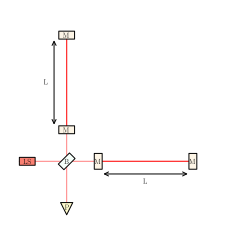
\includegraphics[width=.4\textwidth]{../figures/simple_detector.pdf}
%    \caption{Simplified schematic diagram of an L-shaped GW detector. The labels denote the following objects. LS: Source of laser. B: Beam splitter. M: Mirror. P: Photodiode. The arm length is marked by L which is the distance between the input and output mirror in the given arm.}
%    \label{fig:det_l}
%\end{figure}
\begin{figure}%{l}{0.5\textwidth}  % 'r' for right, 'l' for left
    \centering
    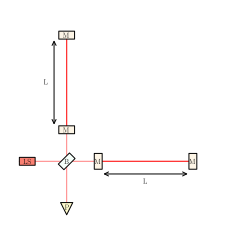
\includegraphics[width=0.38\textwidth]{../figures/simple_detector.pdf}
    \caption{Simplified schematic diagram of an L-shaped GW detector. The labels denote the following objects. LS: Source of laser. B: Beam splitter. M: Mirror. P: Photodiode. The arm length is marked by L which is the distance between the input and output mirror in the given arm.}
    \label{fig:det_l}
  \end{figure}

Ground-based GW detectors such as LIGO, Virgo, and KAGRA, work on the principles of interferometry. By observing the constructive and destructive interference of two laser beams, they can measure very small changes in length. The configuration of ground-based detectors is that of a modified Michelson interferometer~\cite{LIGOScientific:2014pky}. 

\begin{figure}[h]
    \centering
    \includegraphics[width=\textwidth]{../figures/joint_pattern.pdf}
    \caption{Individual and combined antenna pattern functions of the Virgo detector over the whole sky at the time of arrival of GW170817 (blue marker) signal. The dark (bright) colour marks the regions of low (high) sensitivity. The marker shows the median value of the sky-location measurement of GW170817. We note that GW170817 is the closest to Earth and most precisely localised GW source to date (28 deg$^2$ for $90\%$ confidence interval and $40^{+8}_{-14}$ Mpc). Such precise measurements are due to all three GW detectors, LIGO-Livingston, LIGO-Hanford, and Virgo, being online at the time of arrival of the signal. Such measurements may not have been possible without a \textit{network} of GW detectors.}
    \label{fig:antenna_pattern}
\end{figure}
\subsection{Current generation detectors}
A schematic diagram of an L-shaped interferometer is shown in Figure~\ref{fig:det_l}. A laser beam is split into two and travels through two arms of equal length. The light bounces back from the mirror at the end of the arm. The laser travels an equal distance in each arm in the absence of external disturbances, e.g. absence of a gravitational wave. When a gravitational wave passes by, it periodically stretches and squeezes the arms so the light no longer travels the same distance in both arms. By observing the constructive and destructive interference pattern in the light collected by the photodiode, we can measure the strain of the gravitational wave signal. The strain denoted by $h(t)$ is equal to the relative change in arm length denoted by $L$,
\begin{equation}
 h(t) =  \frac{\Delta L}{L}.
\end{equation}

GW detectors are sensitive to the following linear combination of plus and cross polarizations of a GW signal:
\begin{equation}
 h(t) =  \frac{\Delta L}{L} = F_+h_+(t) + F_{\times}h_{\times}(t).
\end{equation}

Here, $F_+$ and $F_{\times}$ are called antenna pattern functions of the detector. They enable the projection of the GW polarizations from the source frame to the detector frame. Unlike conventional electromagnetic telescopes, the GW detectors are not pointed in any certain direction. Their orientation changes only with the rotation of the Earth. Their sensitivity around the sky indeed depends on the sky location, the polarization angle of the gravitational wave, and the arrival time of the signal at the detector. Each $F_i$ is a function of four parameters
\begin{equation}
 F_i := F_i(\alpha, \delta, \psi, t_c),
\end{equation}
where $\alpha$ and $\delta$ denote the right ascension and declination, respectively. The polarization angle is denoted by $\psi$ and time of arrival by $t_c$. Their sensitivity is periodic over $\sim$24 hours. The index $i$ represents the two polarizations.

Figure~\ref{fig:antenna_pattern} shows the antenna pattern functions of the Virgo detector~\cite{VIRGO:2014yos}. We plot the $F_+$ and $F_{\times}$ over the whole sky by varying right ascension from $-180^\circ$ to $180^\circ$ and declination to $-90^\circ$ to $90^\circ$, at the time of arrival of the first gravitational wave signal detected from the merger of two neutron stars also known as GW170817~\cite{LIGOScientific:2017vwq}. We fix the polarization angle to the median value of its polarization angle of GW170817 while creating Figure~\ref{fig:antenna_pattern}.  

\subsection{Third generation detectors}
\begin{figure}[t]
    \centering
    \includegraphics[width=.75\textwidth]{../figures/triangle_detector.pdf}
    \caption{A simple layout of the triangular design of Einstein Telescope. It consists of 3 V-shaped interferometers with an opening angle of 60 degrees, forming an equilateral triangle with an arm-length of 10 km. The object notations are the same as those shown in the L-shaped interferometer, namely, M denotes the mirrors, B denotes the beam splitters, LS denotes the laser sources, and P denotes the photodiodes.}
    \label{fig:triangle}
\end{figure}
The two LIGO detectors~\cite{LIGOScientific:2014pky}, the Virgo detector~\cite{VIRGO:2014yos}, the KAGRA detector~\cite{Aso:2013eba}, and the upcoming LIGO detector in India~\cite{Saleem:2021iwi} are collectively referred to as the current generation or second generation (2G) detectors. While the current generation GW detectors have opened a new window onto the Universe, the proposed third-generation (3G) detectors are expected to usher in an era of precision science. These include the Cosmic Explorer~\cite{Reitze:2019iox} and the Einstein Telescope (ET)~\cite{Punturo:2010zz, ET:2019dnz}. Design and site-selection studies to maximize the scientific potential of 3G detectors are currently underway. 

In particular, Figure~\ref{fig:triangle} shows a simple layout of the proposed triangular design of the Einstein Telescope. The Einstein Telescope is a network of three V-shaped interferometers with an opening angle of 60 degrees, forming an equilateral triangle. The proposed arm-length is 10 km and the infrastructure is expected to be 250 to 300 meters below the ground. At the time of writing of this thesis, the proposed sites for the ET include the Euregio Meuse-Rhine (EMR) located near the border of the Netherlands, Belgium, and Germany, the Sardinia island located in the south-west of Italy, and the Lusatia region in Saxony. Alternate proposals for the configuration of ET include two distant L-shaped detectors (Figure~\ref{fig:det_l}) with 15-kilometre arm-length located in Sardinia and EMR region each~\cite{Branchesi:2023mws}. 

